\title{CS3210 Parallel Computing\\Assignment 2 Report\\[3ex]\textbf{Discrete Particle Simulation with MPI}}
\author{Keven Loo Yuquan (A0183383Y) \& Lee Yong Jie, Richard (A0170235N)}
\date{}

\documentclass[12pt]{article}

% Margins
\usepackage[margin=2cm]{geometry}
% Math and symbols
\usepackage{amsmath}
\usepackage{amssymb}
% Syntax highlighting
\usepackage{minted}
% Inclusion of pictures
\usepackage{graphicx}
\graphicspath{{./reportAssets/}{./processedGpuResults/}}
% Better looking underlines
\usepackage{soul}
\setuldepth{Parallel}
% Combine texttt & textbf
\usepackage{bold-extra}
% No paragraph indentations
\setlength{\parindent}{0pt}
% Merge rows of table
\usepackage{multirow}
% Fixed tables
\usepackage{tabularx}
% LaTeX is dumb at deciding where figures should go
\usepackage{float}
% Enable support for coloured text blocks
\usepackage[dvipsnames]{xcolor}
% Enable URLs
\usepackage{hyperref}
% Enable references on the TOC
\usepackage[nottoc,numbib]{tocbibind}

% \bf formats a chunk of text to both texttt and textbf
\newcommand{\bt}[1]{\texttt{\textbf{#1}}}
% Center-aligned column
\newcolumntype{C}{>{\centering\arraybackslash}X}

\begin{document}
\maketitle
\setcounter{tocdepth}{1}
\tableofcontents

\pagebreak
\large{}
\section{MPI Program Design}

The discrete particle simulation is implemented fully in MPI. The overall architecture of the simulator is summarised in Figure \ref{fig:simulator-design} below. \\

\begin{figure}[H]
    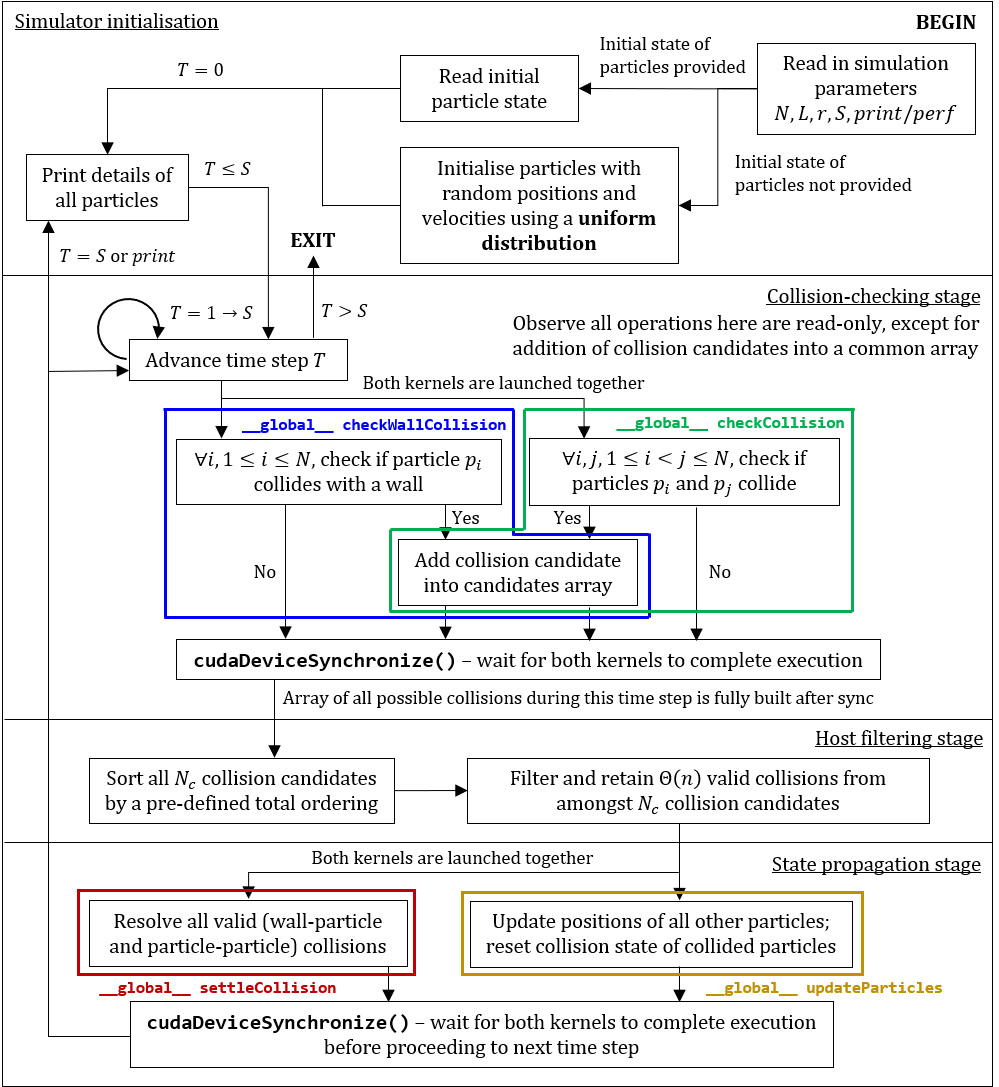
\includegraphics{chap1Flowchart-CUDA}
    \centering
    \caption{Overall simulator design for CUDA implementation}
    \label{fig:simulator-design}
\end{figure}

\pagebreak

\section{Implementation Assumptions and Details}

\subsection{Assumptions}

The first assumption from the earlier report has been removed due to changes in the testing conditions.

\begin{enumerate}
	\item A particle is involved in no more than one collision per time step.
	\begin{itemize}
		\item Implications
		\begin{enumerate}
			\item If a particle collides with a wall after any collision, it is placed at the wall at the end of that time step, and will immediately collide with the wall at the beginning of the next time step
			\item If particle $P$ collides with a particle $Q$ after any collision, it will phase through the particle $Q$ for the remainder of this time step, or will ignore $Q$ the next time step if they happen to overlap
		\end{enumerate}
	\end{itemize}
	\item All collisions between particles and with the wall are elastic (kinetic energy and momentum are conserved). 
	\item It is possible to fit all $N$ particles of radius $r$ into the square of length $L$ without overlapping.
	\begin{itemize}
		\item Implication
		\begin{enumerate}
			\item The simulation exits if one of these two conditions fail: $L < 2r$ (not possible to fit a single particle) or $Nr^2 > L^2$ (not possible to pack $N$ particles in a \ul{grid arrangement} in a square with area $L^2$)
		\end{enumerate}
	\end{itemize}
	\item The set of possible collisions $C$ satisfies a \textbf{total ordering}.
	\begin{itemize}
		\item Implication
		\begin{enumerate}
			\item For each time step $T$, it is possible to sort all collision candidates by this total ordering to determine which collisions should be prioritised over others.
		\end{enumerate}
	\end{itemize}
\end{enumerate}

\pagebreak

\subsection{Implementation Details}

Changes in general implementation details from the previous report are in \textcolor{blue}{blue}.

\begin{enumerate}
	\item If the initial state of particles are not provided, particles are generated with initial random positions and velocities using a \textbf{uniform distribution}.
	\begin{enumerate}
		\item We use the pseudo-random number generator function \texttt{rand} in the C library seeded with the number 3210.
		\item Particles are placed randomly in the square without overlapping.
	\end{enumerate}
	\item Each particle keeps track of its own state: $\textrm{ID}, x, y, v_x, v_y, \textcolor{blue}{w_c, p_c}$.
	\item Our simulation has an additional parameter \texttt{SLOW\_FACTOR} in \texttt{simulator.cu} that increases the granularity of the simulation for greater accuracy. \label{slow-factor-ref}
	\begin{enumerate}
		\item Setting \texttt{SLOW\_FACTOR} to an integer $>1$ slows the initial velocities of all particles by that factor. \texttt{SLOW\_FACTOR} should be set to a power of two to avoid introducing additional floating-point errors when dividing the particles’ velocities.
		\item The number of steps of the simulation is multiplied by \texttt{SLOW\_FACTOR} to compensate, i.e. each original step now corresponds to \texttt{SLOW\_FACTOR} ``micro-steps".
	\end{enumerate}
	\item Collisions are of two types: particle-wall collisions or particle-particle collisions. We describe a particle-wall collision as ($P$, \texttt{null}) and a particle-particle collision as ($P$, $Q$).
	\begin{enumerate}
		\item As particle-particle collisions are symmetric (i.e. $P$ collides with $Q$ $\iff$ $Q$ collides with $P$), we generate these collisions such that $P$ is the particle with lower integer ID \textcolor{blue}{to avoid duplicates}.
	\end{enumerate}
	\item When sorting collision candidates with the C library function \texttt{qsort}, we enforce this total ordering in the function \texttt{cmpCollision}. For two collision candidates  $C_1$ and $C_2$,
	\begin{itemize}
		\item[$\blacksquare$] $C_1 < C_2$ if $C_1$ occurs before $C_2$ \textcolor{blue}{(priority by time)}
		\item[$\blacksquare$] If $C_1$ and $C_2$ occur at the same time
		\begin{itemize}
			\item[$\square$] $C_1 < C_2$ if ID of $P$ in $C_1$ $<$ ID of $P$ in $C_2$ \textcolor{blue}{(priority by ID)}
			\item[$\square$] If $C_1$ and $C_2$ both involve the same particle $P$
				\begin{itemize}
					\item[$\blacksquare$] $C_1 < C_2$ if $C_1$ is a wall collision \textcolor{blue}{(priority by type)}
					\item[$\blacksquare$] If $C_1$ and $C_2$ are both particle-particle collisions
						\begin{itemize}
							\item[$\square$] $C_1 < C_2$ if ID of $Q$ in $C_1$ $<$ ID of $Q$ in $C_2$ \textcolor{blue}{(priority by ID)}
						\end{itemize}
				\end{itemize}
		\end{itemize}
	\end{itemize}
	\item For each particle in each time step, we check once if the particle collides with any of the four walls.
	    \begin{enumerate}
	        \item \textcolor{blue}{A particle is treated to have collided with a wall if it would come within a distance of $\epsilon = $ \texttt{1E-8} to the wall within that time step.}
	    \end{enumerate}
	\item All possible particle-particle collision pairs are checked for each time step. The total number of collision checks performed is thus
	\begin{align*}
	N_{potential\ collisions} 	&= N_{wall-particle} + N_{particle-particle} \\
						&= N + \frac{N(N-1)}{2} \\
						&= \Theta (N^2)
	\end{align*}
	\item Particle-wall collisions are checked by solving the trajectory equation of a particle and the position equations of the wall. The equations of the walls are $x = 0, x = L, y = 0, y = L$.
	\item \label{trajectory-calc} Particle-particle collisions are checked by solving trajectory equations of two particles during the given time step.\\
	
	Consider two particles $P$, $Q$ during a given time step $0 \leq \Delta t \leq 1$. From Pythagoras’ theorem, the distance between them is
	$$d = \sqrt{\left( \left( x_Q + v_{xQ} \Delta t \right) - \left( x_p + v_{xP} \Delta t \right) \right)^2 +
		\left( \left( y_Q + v_{yQ} \Delta t \right) - \left( y_p + v_{yP} \Delta t \right) \right)^2}$$
	or re-written in terms of deltas (differences in state)
	$$d = \sqrt{\left( \Delta x + \Delta v_x \Delta t \right)^2 +
		\left( \Delta y + \Delta v_y \Delta t \right)^2}$$
    \\
	The particles intersect when $d = 2r$, i.e. the particles touch at their circumference, hence by expanding and collecting terms we get the quadratic equation of form $A (\Delta t)^2 + B \Delta t + C = 0$,
	\begin{align*}
		\Delta x^2 + 2 \Delta x \Delta v_x \Delta t + \Delta v_x^2 (\Delta t)^2 + \Delta y^2 + 2 \Delta y \Delta v_y \Delta t + \Delta v_y^2 (\Delta t)^2 &= (2r)^2 \\
		\implies (\Delta v_x^2 + \Delta v_y^2) (\Delta t)^2 + (2 \Delta x \Delta v_x + 2 \Delta y \Delta v_y) \Delta t + (\Delta x^2 + \Delta y^2 - 4r^2) &= 0
	\end{align*}
	
	We observe that $A = (\Delta v_x^2 + \Delta v_y^2) > 0$ and thus the curve $y = d(\Delta t)$ is concave up. The discriminant for this quadratic equation, $B^2 - 4AC$, is
	$$\textrm{discriminant} = (2 \Delta x \Delta v_x + 2 \Delta y \Delta v_y)^2 - 4(\Delta v_x^2 + \Delta v_y^2)(\Delta x^2 + \Delta y^2 - 4r^2)$$
	
	If this discriminant is $\geq 0$, then the particles collide for some value of $\Delta t$, and we solve for this $\Delta t$. There are two possible roots,
	$$\Delta t = \frac{-B \pm \sqrt{\textrm{discriminant}}}{2A}$$
	
	Since the quadratic curve is concave up, we only compute and examine the first root (when the particles are approaching each other). This is
	$$\Delta t = \frac{-B - \sqrt{\textrm{discriminant}}}{2A}$$
	
	If $0 \leq \Delta t \leq 1$, then particles $P$, $Q$ collide during this time step.
	
	Note that, it is possible for $\Delta t < 0$ - this corresponds to cases where particles are overlapping from a previous step. We do not consider these as collisions in the current step and let these two particles phase through each other.
	\item \textcolor{blue}{To ensure the collision candidates array can accommodate $\Theta(N^2)$ potential collisions (in the limit of large $N$ when particle-particle collisions dominate), we dynamically allocate an array in managed memory with sufficient space to store $N^2 / 2$ collision structs.}
	\begin{itemize}
	    \item \textcolor{blue}{Unfortunately, \texttt{cudaMallocManaged()} fails to allocate the required space when $N = 64000$.}
	\end{itemize}
\end{enumerate} 

\pagebreak

\section{Assignment 1B (CUDA) addendum: Float performance on the NVIDIA Titan V GPU}

Some words here.

\begin{figure}[H]
    \centering
    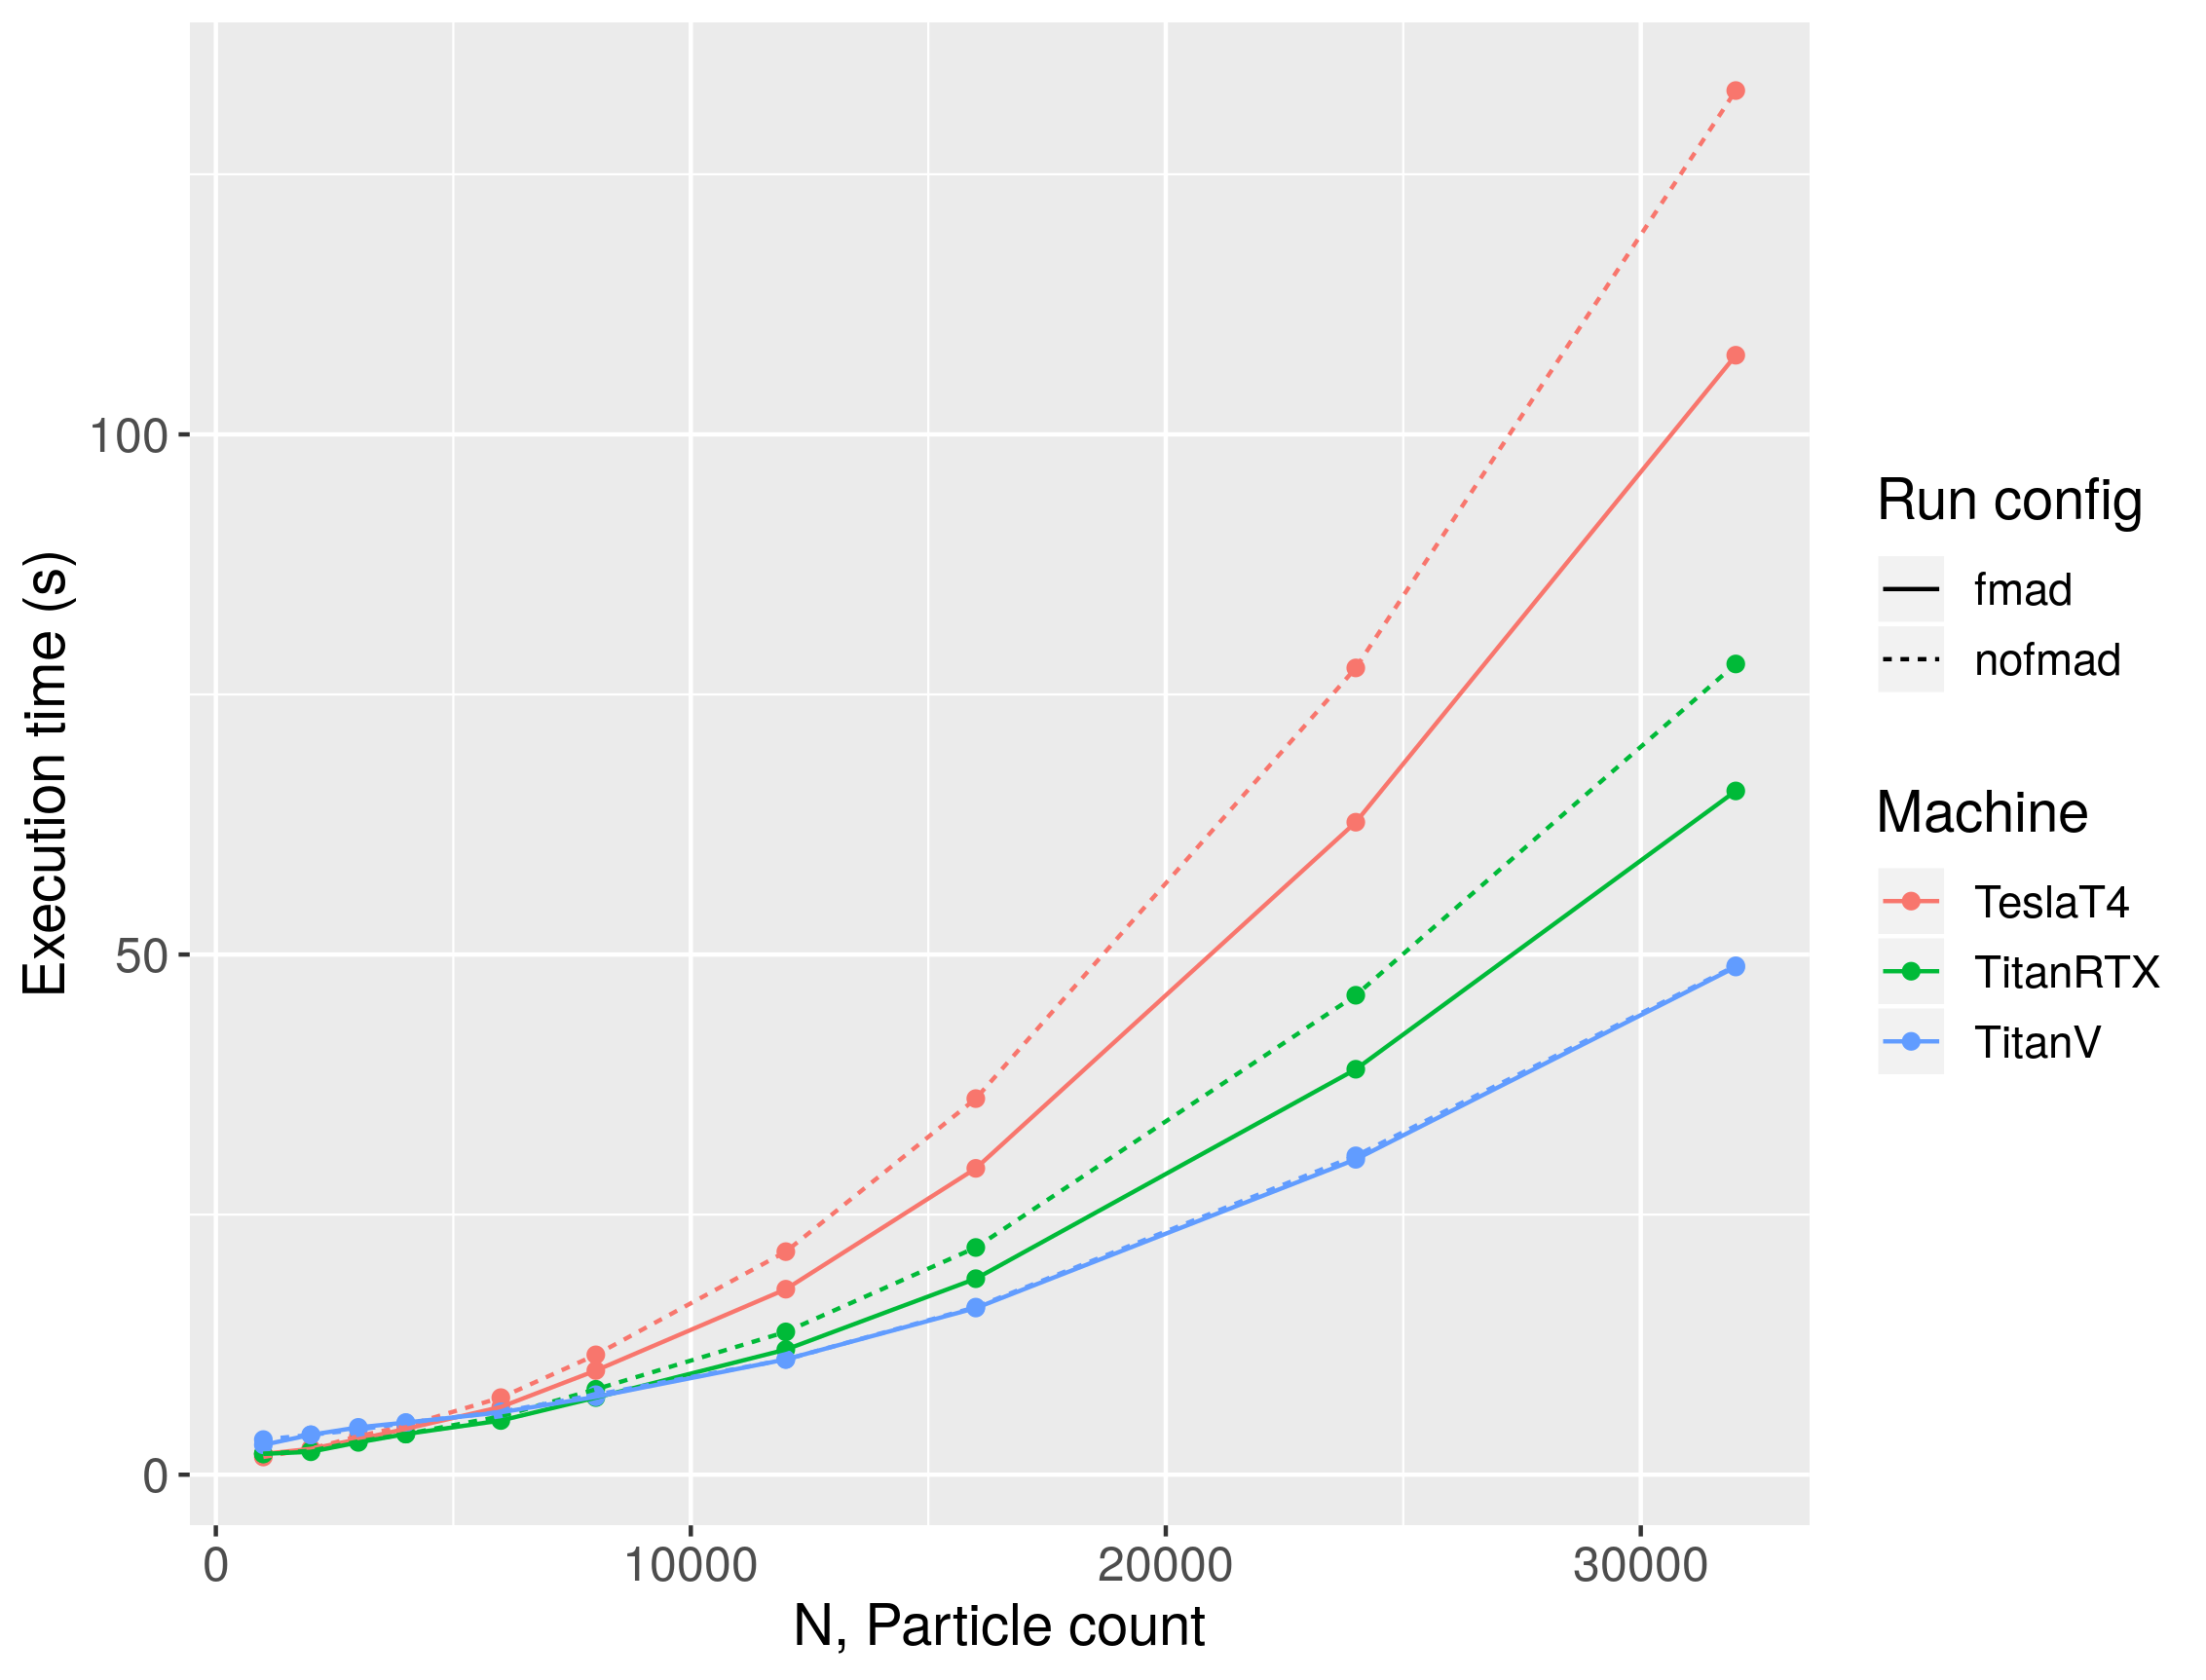
\includegraphics[width=0.75\textwidth]{gpu-varyN}
    \caption{Plot of execution time against particle count, $N$}
    \label{fig:gpu-varyN}
\end{figure}

\begin{figure}[H]
    \centering
    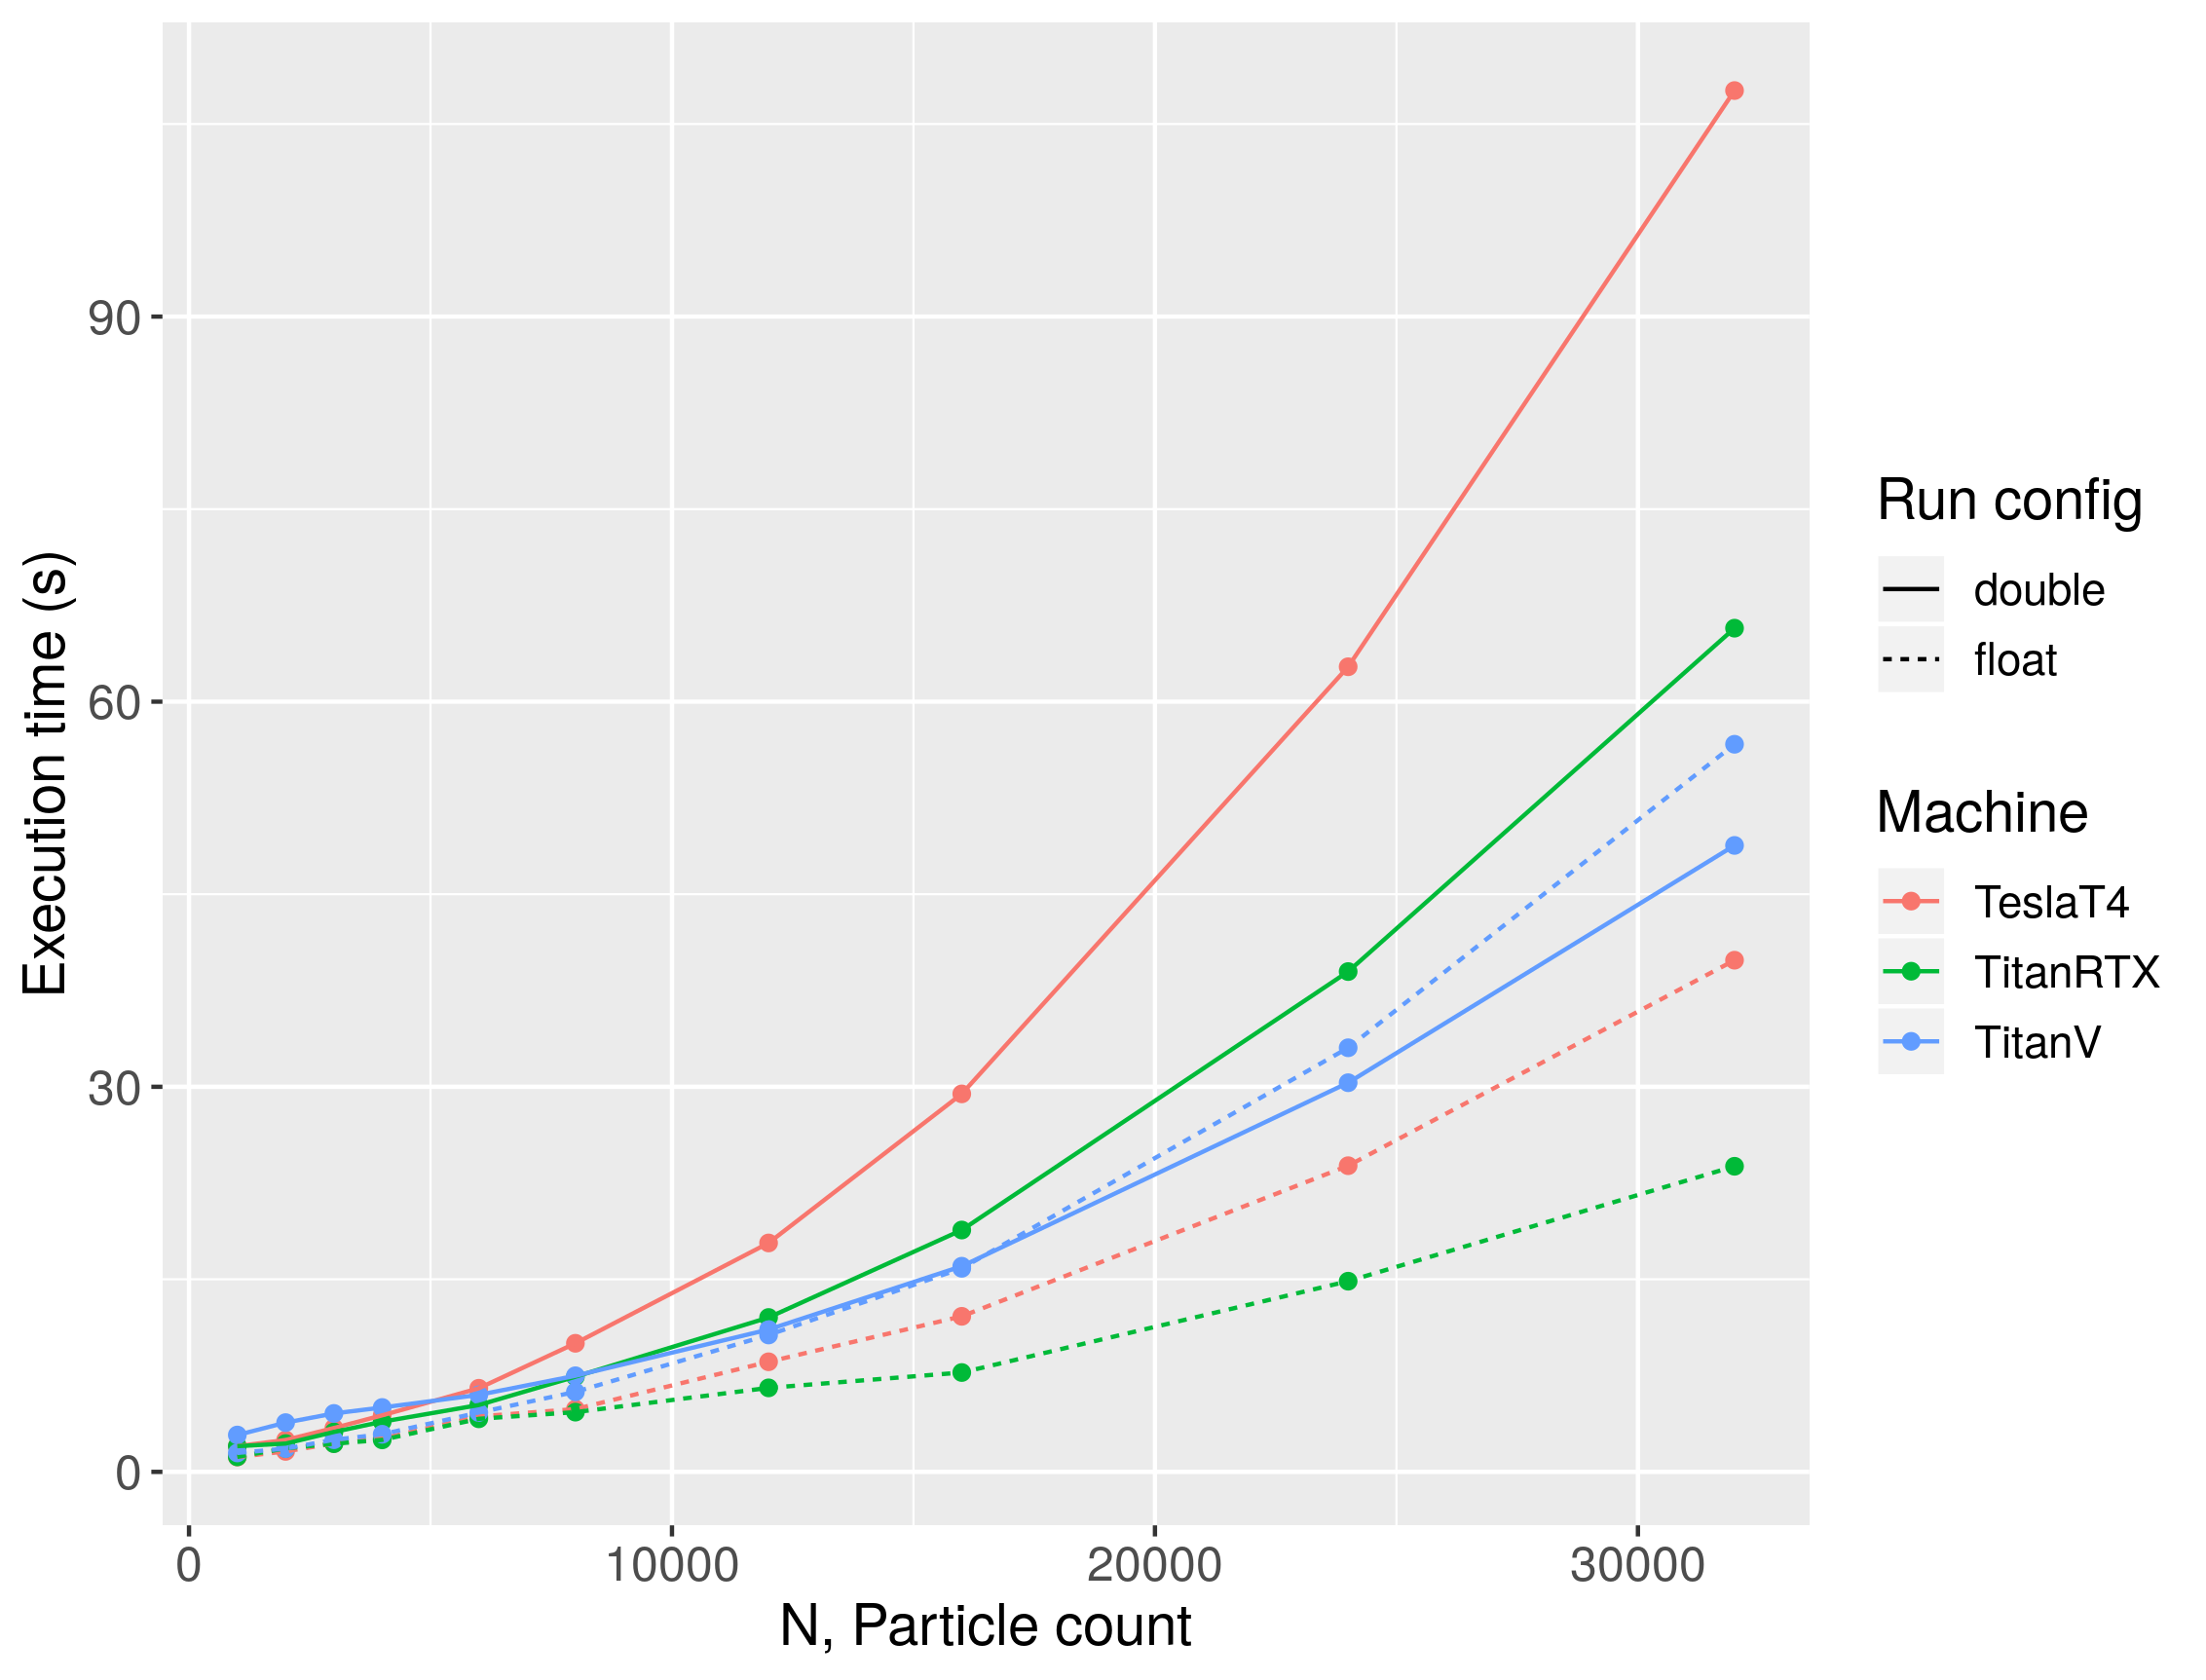
\includegraphics[width=0.75\textwidth]{double-float-comparison-fmad}
    \caption{Plot of runtime (s) against $N$ for \texttt{float} and \texttt{double} programs (\texttt{--fmad=true})}
    \label{fig:double-float-comparison-fmad}
\end{figure}

\begin{figure}[H]
    \centering
    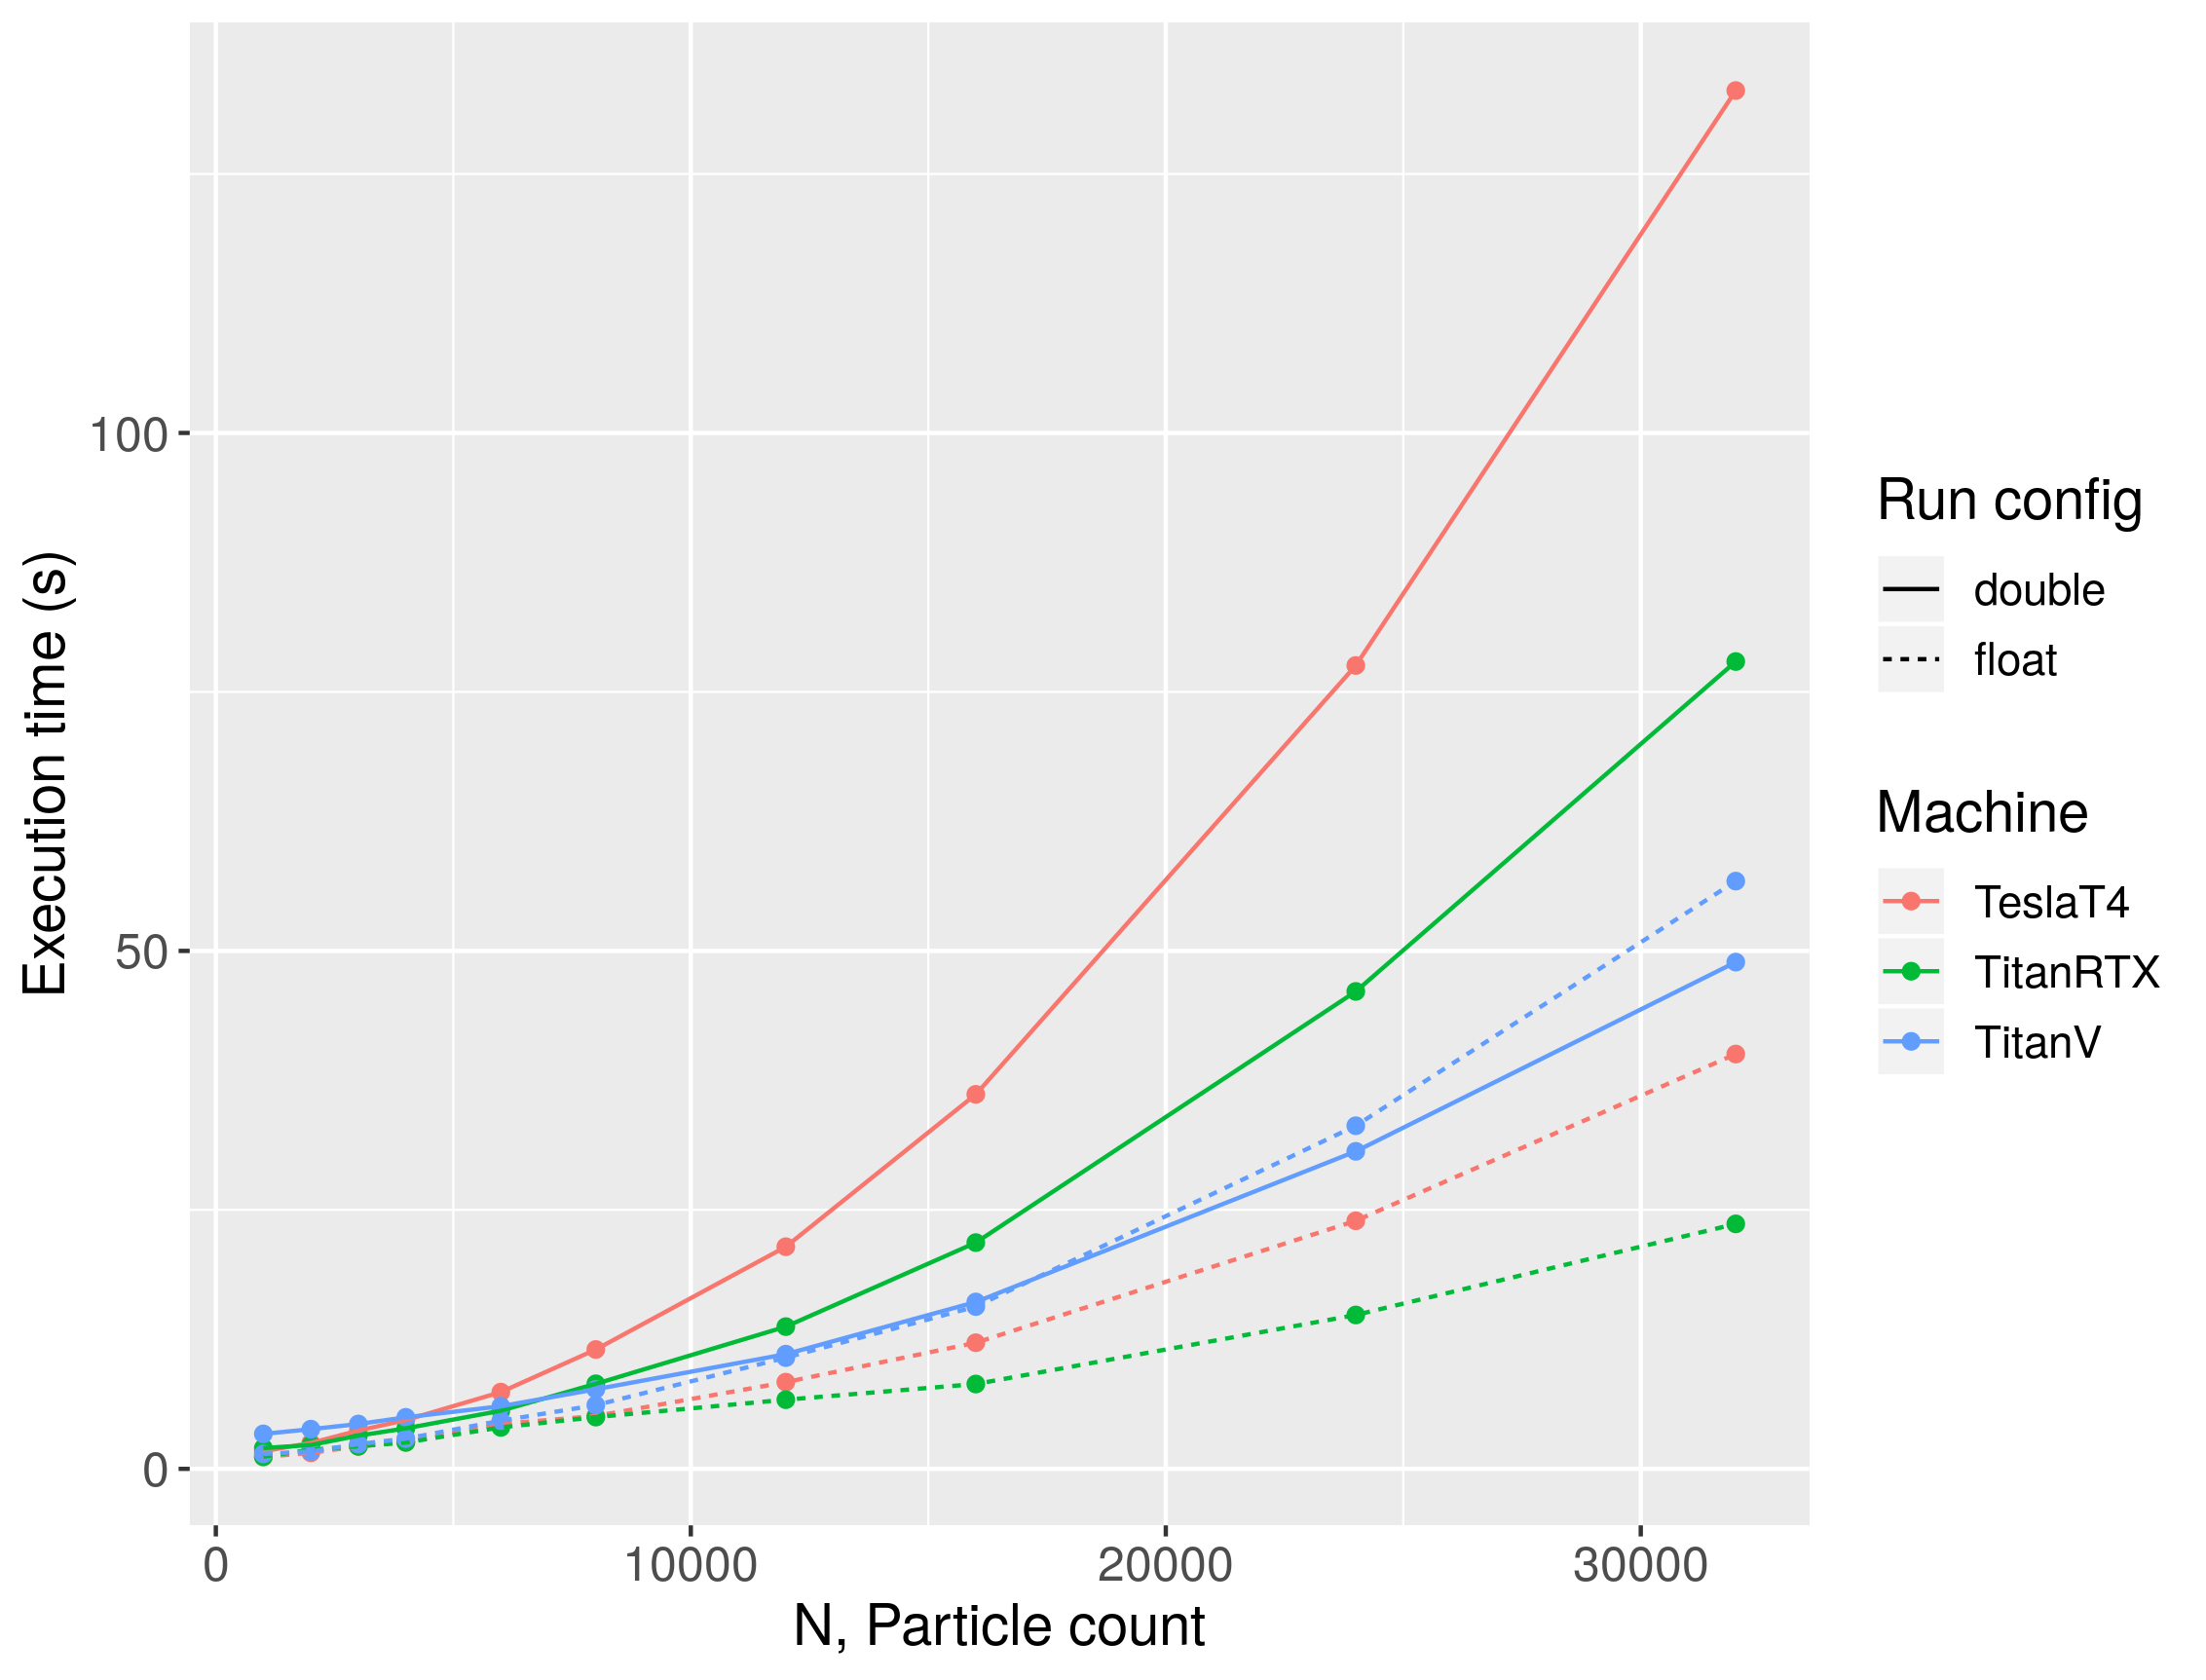
\includegraphics[width=0.75\textwidth]{double-float-comparison-nofmad}
    \caption{Plot of runtime (s) against $N$ for \texttt{float} and \texttt{double} programs (\texttt{--fmad=false})}
    \label{fig:double-float-comparison-nofmad}
\end{figure}

\section{Filler section}

We cite our previous assignments, 1A \cite{assign1aref} and 1B \cite{assign1bref} for no apparent reason. Who knows, we might reference them soon.

\pagebreak

\bibliography{references}
\bibliographystyle{abbrv}

\end{document}